\documentclass[11pt]{article} % use larger type; default would be 10pt
\usepackage[utf8]{inputenc} % set input encoding (not needed with XeLaTeX)

%%% PAGE DIMENSIONS
\usepackage{geometry} % to change the page dimensions
\geometry{a4paper} % or letterpaper (US) or a5paper or....
\newcommand{\tab}{\hspace*{2em}}

%%% PACKAGES
\usepackage{graphicx} % support the \includegraphics command and options
\usepackage{wrapfig} % Figure wrapping
% \usepackage[parfill]{parskip} % Activate to begin paragraphs with an empty line rather than an indent
\usepackage{booktabs} % for much better looking tables
\usepackage{array} % for better arrays (eg matrices) in maths
\usepackage{paralist} % very flexible & customisable lists (eg. enumerate/itemize, etc.)
\usepackage{verbatim} % adds environment for commenting out blocks of text & for better verbatim
\usepackage{subfig} % make it possible to include more than one captioned figure/table in a single float
\usepackage{url}
\usepackage{enumerate}
\usepackage{cleveref}  %cites figures intelligently
\usepackage{import} % document structuring
\usepackage{float}  %These two ensure that table position follows text by specifying {table}[H]
\restylefloat{table}

%CODE LISTINGS
\usepackage{color}
\usepackage{listings}

\lstset{
	tabsize=4,
%	language=matlab,
        	basicstyle=\scriptsize,
%     	upquote=true,
       	aboveskip={\baselineskip},
        	columns=fixed,
        	showstringspaces=false,
        	extendedchars=true,
        	breaklines=true,
	prebreak = \raisebox{0ex}[0ex][0ex]{\ensuremath{\hookleftarrow}},
	frame=single,
        	showtabs=false,
        	showspaces=false,
        	showstringspaces=false,
        	identifierstyle=\ttfamily,
        	keywordstyle=\color[rgb]{0,0,1},
        	commentstyle=\color[rgb]{0.133,0.545,0.133},
        	stringstyle=\color[rgb]{0.627,0.126,0.941},
	language=C++
}

%%% HEADERS & FOOTERS
\usepackage{fancyhdr} % This should be set AFTER setting up the page geometry
\pagestyle{fancy} % options: empty , plain , fancy
\renewcommand{\headrulewidth}{0pt} % customise the layout...
\lhead{}\chead{}\rhead{}
\lfoot{}\cfoot{\thepage}\rfoot{}

%%% SECTION TITLE APPEARANCE
\usepackage{sectsty}
\allsectionsfont{\sffamily\mdseries\upshape} % (See the fntguide.pdf for font help)
\usepackage{titlesec}
%\titleformat{\subsection}[runin]{\mdseries\bf}{\thesubsection}{1em}{}
%\titleformat{\subsubsection}[runin]{\mdseries\bf\underline\large}{\thesubsection}{1 em}{\vspace{-5 pt}}

\usepackage{footbib}

% (This matches ConTeXt defaults)

%%% ToC (table of contents) APPEARANCE
%\usepackage[nottoc,notlof,notlot]{tocbibind} % Put the bibliography in the ToC
\usepackage[titles,subfigure]{tocloft} % Alter the style of the Table of Contents
\renewcommand{\cftsecfont}{\rmfamily\mdseries\upshape}
\renewcommand{\cftsecpagefont}{\rmfamily\mdseries\upshape} % No bold!

\begin{document}
%% END Article customizations



\part{Motion Detector}
\paragraph{A Motion Detector is a camera device that uses hardware or software to detect a significant change between scenes and flag that movement has occurred. The first motion detector was invented by Samuel Bagno in the 1950s as a burglar alarm, making use of ultrasonic waves to measure the Doppler change in frequencies to measure movement. Modern day motion detectors make use of the same technology; using infrared to measure changes in heat, or microwave lasers to measure the distance of a scene.\\
Mobile phone's however do not come equipped with microwave lasers nor ultrasonic emitters, and though a significant amount of mobile phones have infra-red sensors and bluetooth radio sensors, the poor resolution of these sensors makes using them as reliable motion detectors somewhat tricky.\\
Modern smartphones of today do often come equipped with camera's whose images can be used to detect motion, but all the processing is done in the software which can be slow. Fortunately smartphones of today are fast enough to handle such image processing, and using lower-level languages such as C and C++ the strain on the phone can be greatly reduced.}

\section{Competition}
\paragraph{Due to the small community of Maemo users, there are not many apps of this nature on the platform and thus not much competition at all.}

\section{Software Battles}
\paragraph{To start a basic motion detector, the very least that I would need to do is take one frame and subtract it from another to see the difference. To do this I would need to store every pixel value in an array for each image and then perform a sweep over both arrays to compare their pixel values. There must be imaging libraries that I could use that would greatly facilitate such imaging techniques. But first I would need to be able to take a single photo.....}

\subsection{QtMobility vs Gstreamer vs FCam}

{\bf QtMobility} is a Qt library that enabed developers to have access to standard mobile functionality such as messaging, contacts, multimedia, and camera.  The camera is contained within a QCamera widget and simple calls can be made to the imaging device.
\\Unfortunately the official stable version v1.1 had camera support for Symbian and Meego(Harmattan), but not Fremantle. There was an unstable version 1.2 which included Fremantle support, but once I had installed libqtm-dev\_1.2 on the rootstrap device, and tried to use the QCamera element from within a C++ class it did not work. This is because the QCamera element has to be accessed through QML, which would be doable but would not be optimized for speed. For this reason I dropped QtMobility.

{\bf GStreamer} is an open source multimedia framework that is already native to Fremantle since it is the library that the default mediaplayer uses and so would reduce the dependencies of my application. GStreamer makes use of pipelining, byt connecting a number of elements in an ordered fashion so that the output (source) of one element is fed into the input(sink) of another element and so on until it reaches the final element which is usually a file or a network stream.
\\\\A previous app of mine was Gstreamer based and a typical command from it would be:
\label{gstreamer}
\begin{verbatim}
	      gst-launch v4l2src device=/dev/video0 ! \
	      videoscale ! video/x-raw-yuv, width=320, height=240 ! \
	      ffmpegcolorspace !  jpegenc 80 ! \
	      tcpserversink host=192.168.1.101 port=9000
\end{verbatim}

This pipes the video-for-linux(version2) camera source into a video scaling element, into a raw video stream of defined height and width, into an element that convert the pixel color depths to type ffmpeg color sizes, into an element that encodes the raw stream into mjpeg format with a quality of 80\%, which then pipes it into a tcp server element which broadcasts to the specified host and port.
\\On the recieving side, a gstreamer pipe would need to reverse the order of the elements (i.e. recieve from tcpserver, feed it into a jpeg decoder, and then specify an output window or file sink.
\\Gstreamer is very well developed, and has a Good, Bad, and Ugly heirarchy of stable to unstable plugins that can be used to enable a wide array of different multimedia functionalities and formats.

Despite the speed and efficient usage of system resources, GStreamer has an extremely involved API but is difficult to work with since it is prone to cascading errors due to the every element being dependant on the previous element to function. An example of the C++ implementation of the same code as above is shown in the appendix.\\

FrankenCamera (or {\bf FCam}) is a very easy to use open-source C++ API for controlling digital cameras.  The FCam architecture was developed as a joint reasearch project between Stanford Computer Graphics and Nokia's Research Center for controlling the N900's camera, but has since been used to run their own F2 camera built in their labs\footcite{fcamdoc}. Normally camera architectures are not so easily accessible and it is very fortunate that FCam chose the N900 to develop on.
\pagebreak
\\The FCam API is split into 4 components:
\begin{enumerate}
\item[Device]{The camera device consists of a Lens, a Flash and other different devices. FCam has object classes for each of these with various functionlity enabled.}
\item[Shot]{The shot object holds typical parameter settings such as exposure time, frame time, white balance, and gain for capturing and processing a single image. It is applied to the sensor object.}
\item[Sensor]{The sensor object listens for calls for capture, and outputs a frame by performing all the image pipelining in it's own thread. Once pipeline exits (or the thread terminates) the sensor is ready to be configured for the next frame.}
\item[Frame]{Frames can be accessed from the sensor by calling the getFrame() function which performs blocking on any pending shots. The ease of API is shown here, as this is the \it{only} blocking call in the entire API.}
\end{enumerate}

\begin{wrapfigure}{R}{0.5\textwidth}
	\vspace{-40pt}
	\begin{center}
		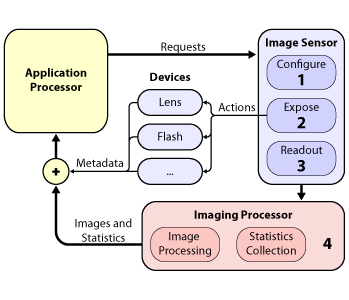
\includegraphics[width=0.5\textwidth]{../images/fcam_arch}
	\end{center}
	\vspace{-20pt}
	\caption{FCam Architecture}
\end{wrapfigure}
It has an extremely simple API, since all the user has to do is set the shot parameters, call a new frame, and grab the image from the frame. This can be called any times in succession using the same parameters with comparitavely little lines of code.\\
Despite being a relatively small project, the API was extremely detailed and had many examples that I could adopt. For these reasons, FCam was the acrhitecture used for the developement of this project.

To use it, I had to add an -lfcam dependency to the LIBS+= heading in the .pro file, and fcam-dev\_1.2.deb had to be installed to the rootstrap device.\\

FCam has different image sizes depending on the colorspace of the frame that it is being extracted from. For example RAW formats only allow an aspect ratio of 4:3 (2592x1968, 1296x984, 648x492, ...160x120). However using RAW images may be better for precise image processing, but the memory it uses has a lot of overhead and for frequent repetitive use it is not very practical.

Instead the FCam::UYVY colorspace was adopted which captures the image using three components: Y, U(Cb), and V(Cr). 
Images in this format allow subsampling to reduce the color band resolution (U and V) with a constant brightness (Y) without affecting the image quality discerniable to the human eye. This is because the human eye percieves changes in colour much less significantly than changes in brightness. UYVY format adopts the 4:2:2(Y:U:V) scaling system, where Y is sampled at every pixel and U and V are sampled at every second pixel horinzontally on each line. This greatly reduces the memory size of the image and speeds up processing with very little difference in quality.\\
Supported UYVY image sizes are: (2592x1968, 1280x960, 800x600, 640x480, 320x240, 160x120)

\subsection{OpenCV vs CImg}
\subsubsection{OpenCV}
\paragraph{Now that I had my camera driver configured, I needed to choose an appropriate image library to perform the processing. Technically I could have written my own library class to perform the simple image subtraction and addition functions that I wanted, but there may have been more to offer down the line and I wanted to see what was available. OpenCV and CImg are both common imaging libraries for C, C++, and Python, for use with real-time image proccessing.  Both are used widely in computer vision applications, and both contain approximately the same core capabilities, though OpenCV has more extraneous features.}
\paragraph{The Open Source Computer Vision Library (or OpenCV) was developed by Intel for use with computer vision applications, but since was dropped and is now maintained by Willow Garage and Itseez.
\\OpenCV comes with many useful functions for motion detection: image subtraction, image averaging, normalising, and even its own method for tracking movement. It has an image format called IPLImage and inorder to preform operations I have to convert from FCam's relatively unknown Fcam::Image format to IPLImage. This proved difficult.
}
\paragraph{The FCam Image format is made up of:
FCam::Image::Image(
     int width,
     int height,
     Imageformat f,
     unsigned char* data,
     int srcByesPerRow
)
The IPLImage has BGR channel order (i.e the first channel is blue, second is green, third is red. This is different from standard RGB formats). I attempted to convert to a grayscale IPLImage by doing:}
\begin{frame}[fragile]
\lstinputlisting[title=\textbf{Source Code: IPLconvert.cpp}]{../Code/API_Examples/IPLconvert.cpp}
\end{frame}
\paragraph{as taken from http://www.cs.cornell.edu/courses/cs4670/2010fa/projects/p1/codes/project1.tar.gz\\
This took a reference to the FCam's Frame, extracted the image from it, and attempted to convert it into an unsigned 8-bit gresycale IPL image with 1 color channel. The unsigned 8-bit image would be limited to 0-255 range.\\
Unfortunately several problems were encountered and almost three days were lost trying to get to the bottom of it:}
\paragraph{
A Maemo port of openCV does exist for Fremantle \footcite{libcv} but despite installing libcv, libcv-dev, and many of it's dependencies (libcvcore, libhighgui) the SDK would complain about many missing dependencies when building the application. The culprit turned out to be missing dependencies for libhighgui-dev, but this was false since running a quit dpkg -L \(\langle\)dependency\_name\(\rangle\) confirmed that the dependency was indeed installed. At one stage I copied my entire /usr/lib directory from the phone to the rootstrap but it would still fail when trying to build.\\
A few hours of trawling through the Maemo reading lists came up with a bug report \footcite{highgui-dev} from the original maintainer claiming a bug within the build system.\\
For this reason OpenCV had to be abandoned and a new image processing library had to be used.
}
\subsubsection{CImg}
\paragraph{CImg was suggested by my project supervisor after we discussed the bugs I had been experiencing. CImg is relateivly bug free since it does not exit in any packaged form. In fact all the functions and image processing capabilities are contained within a single 40,000 lined header file coming up to 2.54MB in size. \\Despite the jaw-dropping overhead of including this file in development process, Qt only had to parse the functions within it once and it was set to go.
\\Another bonus is that it removes a dependency from the project, and makes it all that much more portable. One thing I had to do first was to convert from FCam to CImg.
\\The CImg constructor is formed of:\\
CImg(const unsigned int width,\\
\tab const unsigned int height,\\
\tab const unsigned int size\_z=1, //depth\\
\tab const unsigned int size\_c=1 //spectrum\\
)\\
To construct a CImg, all one has to do is call ‘CImg\(\langle\)T\(\rangle\) Name’; where T is the type or size of each pixel value, and name is the name of the image. So for an image that that has 256 colorspace, T = unsigned char = 8bit.
In CIMG, the color channels are in RGB format. OpenCV's IPLImage only supports up to 4 color channels but CImg supports up to any number and this provided a source of initial confusion for me.
http://sph2grid.googlecode.com/svn-history/r14/trunk/CImg/plugins/cimg\_ipl.h:\\
Using the same format as the cornell code I attempted to make:}
\begin{frame}[fragile]
\lstinputlisting[title=\textbf{Source Code: IPLconvert.cpp}]{../Code/API_Examples/CImgConvertBad.cpp}
\end{frame}
\paragraph{This wasn't able to produce a consistent image (or any image at all) and I had to play around a wide variety of pixel values:}
\begin{frame}[fragile]
\lstinputlisting[title=\textbf{Source Code: imagetest.cpp}]{../Code/convert.cpp}
\end{frame}
\paragraph{The idea was that by specifying the (i,j) coordinates of the new image and grabbing the pixel values from the FCam image and sticking it into (i,j) coordinates of the new CImg. I attempted to divide by 255 in some of the tests because I wasn;t sure how large the FCam::Image was, and this was my idea of normalizing it. I later realised that the pixel values were already normalized to 8-bit values and that dividing by 255 limited the CImg to \{0,1\} values would ultimately produce a black image.}
\paragraph{By digging around through the source of the original fcam application for the N900, I was able to find a function that converted FCam by accessing the image data and reading from it:}
\begin{frame}[fragile]
\lstinputlisting[title=\textbf{Source Code: CImgConvertFcam.cpp}]{../Code/API_Examples/CImgConvertFcam.cpp}
\end{frame}
This resulted in images that looked like this:
\begin{center}
\begin{wrapfigure}{R}{0.5\textwidth}
	\vspace{-20pt}
	\hspace{70pt}
		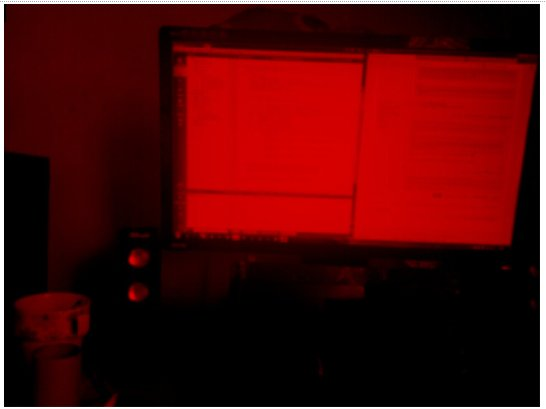
\includegraphics[width=0.5\textwidth]{../images/redbuffer1}
	\vspace{-20pt}
	\caption{Very red image.}
\end{wrapfigure}
\end{center}
\paragraph{
A similar image would appear using imgBuffer[1] instead of imgBuffer[0], and I didn't understand why until I looked up CImg's documentation and realised that out of the 32 channels I was initialising, the first channel is red and that was the only channel I was writing to.
That is, for a greyscale image from 0-255 at pixel i,j - I was sticking it into CImg\{Red,0,0,0,0....32 times.\}, and thus ending up with a red image.
\\Once I limited CImg to 1 color channel (i.e. black and white) then I got my desired image as shown by the real and greyscale comparison below:
}
\begin{wrapfigure}{R}{0.4\textwidth}
	\vspace{-20pt}
	\begin{center}
		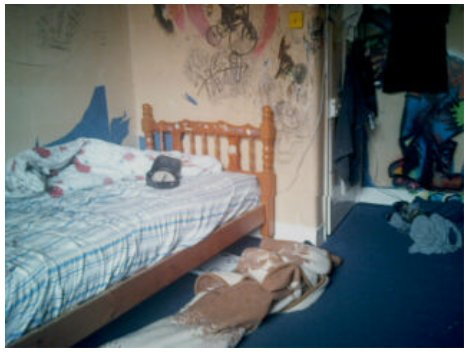
\includegraphics[width=0.4\textwidth]{../images/realbuffer2}
	\end{center}
	\vspace{-20pt}
	\caption{Image saved by FCam}
	\vspace{0pt}
	\begin{center}
		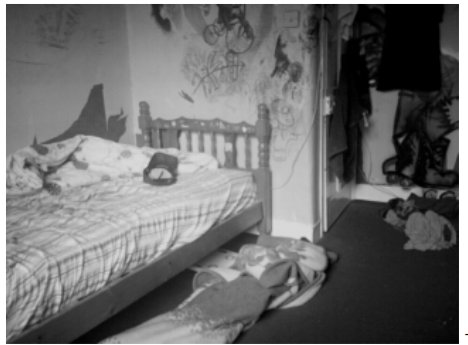
\includegraphics[width=0.4\textwidth]{../images/blackbuffer3}
	\end{center}
	\vspace{-20pt}
	\caption{Image saved by CImg}
	\vspace{-40pt}
\end{wrapfigure}

\subsection{ImageMagick vs FFMpeg vs VLC vs Mencoder}
\paragraph{Now that the image processing side of this was underway, I needed a program that could convert a series of images into a movie format so that when the user returns to their motion detector, they can watch all the highlights in the movie file over the course of a few seconds rather than having to flit through each individual image.
}
\paragraph{Imagemagick is an open-source image software library for processing images. It can perform much of the same functions and CImg and OpenCV, but it was not considered as a suitabe image processing library because the development package had not been released for Maemo and compatibility was a concern. There is, however, a imagemagick package for Maemo that performs the functions from commandline and so accessing its functions would not be a problem if I was resigned to the fact that I would be calling a system process from Qt. CImg has good compatibility with Imagemagick since it's convertToJPEG command actually calls the 'convert' module of Imagemagick.}
\paragraph{
According to the documentation, to convert a series of jpegs to a movie format, all one has to do is call:
'convert -delay \(\langle\)frametime\(\rangle\) input\_jpegs\_*.jpg output\_movie.mpg'\\
But this failed with Maemo specific errors:\\\\}
\begin{frame}[fragile]
\lstinputlisting[title=\textbf{Source Code: Errors}]{../Code/errors.cpp}
\end{frame}
\paragraph{so I was not able to use imagemagick on the device. This is perhaps a good thing since the imagemagick suite is very large and would be a hefty dependency to add to my project
}
\paragraph{FFmpeg was my next and most immediate option - I have used it countless times before to convert movie files and I have found it's libavcodec library a powerful and useful tool in the past. FFMpeg is one of the most popular free multimedia frameworks around, supporting every single codec and format under the sun. It has a fast release time too and when a new format is released it is not usually a long wait before ffmpeg has a supporting library for it. FFmpeg is primarily used to stream, convert, decode, mux, demux and transcode video files into different formats, but is not used for computer vision.\\
For converting a series of images to a movie file the documentation states that one has to call:\\
'ffmpeg -i name\_of\_files\_\%05d.jpg -y movie.mpg -r fps'\\
It is key to note here that the y flag overwrites any output file that already exists, and that the frames-per-second flag '-r' must be placed at the end. The \%05d just notifies FFmpeg that the format for the image files are padded by zeros by up to 5 digits.\\
Despite using different arrangements and different flags, this only partially worked, as the images would be compiled into a movie, but the framerate flag was temperamental and sometimes ignored.\\
Additionally ffmpeg does not come installed as default by the device, since gstreamer is main multimedia framework used by the mediaplayer and this would also be a needlessly large dependency to have for my project
}
\paragraph{VLC is a comparitavely new open-source mediaplayer which can also perform transcoding, streaming, muxing and the same functions as FFMpeg. In fact alot of its codecs are actually taken from the ffmpeg project (e.g. libavcodec), but it also contains a lot of its own.\\
VLC has only been very recenly ported to Maemo and is accessed by adding user Qole's repository to the /etc/apt/sources.list. It is very incomplete, lacking a decent GUI, but it has a working backend. Unfortunately nowhere in the documentation does it mention being able to convert a series of jpegs to a movie file and I soon had to abondon VLC too.\\ This is probably for the best since VLC is not available in the main repositories and users would find it hard to access. This leaves...}
\paragraph{Mencoder is yet another multimedia framework released under GPL, and comes as a module with mplayer, a very stable open-source media player that comes with all the codecs and formats that mencoder can use.\\
To convert a series of images to a movie file one simply has to call:\\
'mencoder "mf://path/to/images*.jpg" -mf fps=\(\langle\)fps\(\rangle\) -o movie.mpg -ovc lavc -lavcopts vcodec=mjpeg'\\
which specifies the that libavcodec is to be used, the framerate and also that the output videocodex should be mpeg format.
\\Mencoder is also not pre-installed with the device, but many Maemo users do tend to install it first chance they get due to the default Media Player's poor support for certain MPG formats, this is by far the most convenient of the four video processing libraries to use and best of all it actaully works.
}
\section{Image Processing Techniques}
\paragraph{A motion detector works on the basic priniciple that there there exists some drastic difference between two images where motion has occred and motion has not occured. One way to see this represenation is to subtract one frame from another and look for the leftover pixels. Pixels where the image hasn't changed will have the same pixel value and will thus cancel each other out, whereas images where there is a difference between pixels at the same location will have values greater than zero. In the case of unsigned chars, any negative pixels will naturally wrap around and becomes high pixel values (white).}
\subsection{Subtraction}
\begin{wrapfigure}{R}{0.3\textwidth}
	\vspace{-40pt}
	\begin{center}
		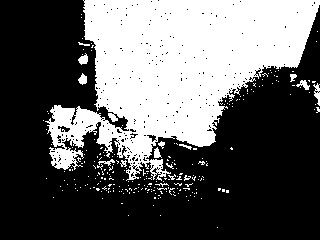
\includegraphics[width=0.3\textwidth]{../images/subG}
	\end{center}
	\vspace{-20pt}
	\caption{Image subtraction between two consecutive frames where the scene has changed inbetween}
	\vspace{10pt}
	\begin{center}
		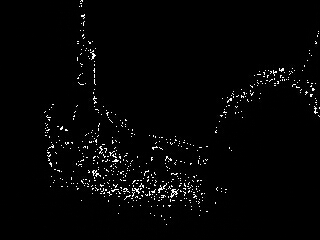
\includegraphics[width=0.3\textwidth]{../images/subF}
	\end{center}
	\vspace{-20pt}
	\caption{Image subtraction between two consecutive static frames where no movement has occured}
\end{wrapfigure}
Subtraction is the technique that performs this, and CImg handles this operation using the basic numerica operator '-', so that for example: CImg\(\langle\)T\(\rangle\) diff = CImg\(\langle\)T\(\rangle\)A - CImg\(\langle\)T\(\rangle\) B;

The images above were normalised to 2 discrete \{0,1\} values and then multiplied by 255 so that the 'hot pixels' could be viewed with the human eye. As you can see from the top figure, the whiteness indeicates that there was a significant difference between frames and so that one of the images had pixel values vastly greater than the other -- indicating a change in the scene.
\\For the bottom image it can be seen that there is very little difference exists between the frames, yet you can almost quite clearly makeout the edge of the objects between the frames (a computer screen and speaker). Neither the speaker, the monitor, nor the camera moved between those two images but nonetheless a small difference was detected.\\
This served as my first model for image detection by performing a small test to see how many of these sparse white pixels are detected for static frames. This would then serve as the basis for a threshold, so that any subtracted frames that are significantly above this threshold are flagged as 'movement' frames and those below or up to the threshold 
are not.
\pagebreak
\subsubsection{Experiment 1: Determining a suitable threshold for subtracted images}
\paragraph{To find a suitable threshold I used the following pseudocode to determine a threshold for a static frame:\\\\}
\begin{frame}[fragile]
	\vspace{-40pt}
	\lstinputlisting[title=\textbf{Source Code: subtract1.pseudo}]{../Code/pseudo/subtract1.pseudo}
\end{frame}
\paragraph{It essentially grabs an image and subtracts it subtracted one image from another and totalled up all the pixels with a value greater than zero. This gave the following table of results:}
\begin{center}
\begin{table}[!htbp]
	\begin{center}
	\begin{tabular}{| c | l | l | l | l | l | }
\hline
\multicolumn{6}{|c|}{\bf Non-Zero Counts from Subtracted Images} \\
\hline
\bf Test	&\bf Scene 1	&\bf Scene 2	&\bf Scene 3	&\bf Scene 4	&\bf Scene 5	\\ \hline
1	&30747	&47298	&37881	&18801	&678\\
2	&9067	&9129	&33326	&7645	&8488\\
3	&798	&35861	&17947	&6433	&444\\
4	&3841	&30449	&8273	&23614	&13385\\
5	&34379	&25246	&6303	&41523	&23474\\
6	&9144	&256	&14960	&31458	&25138\\
7	&333474	&312598	&771731	&33779	&725415\\
8	&34488	&2676	&14522	&1256	&12165\\
9	&36351	&12497	&472	&1036	&18955\\
10	&6133	&23077	&12343	&31430	&25410\\ \hline
\bf Average	&49842.2	&49909	&91776	&19698	&85355\\ \hline
	\end{tabular}
	\end{center}
	\caption{}
	\label{tab:sub1}
\end{table}
\end{center}
\paragraph{as shown in \Cref{tab:sub1} the Average white pixel count is extremely high and varies greatly from scene to scene. Setting a threshold of less than 90000 would work for the five different scenes tested in my experiment, but there’s no gauruntee that the fluctuation between frames would not be higher than 90000 for another scene. \\
So Why is there so much fluctuation? For one, the average pixel values of one scene can be radically different to another scene. If the average pixel value for Scene1 is 45 and the average pixel value for Scene2 is 90, then assuming that the ambient light in a scene is decreased by 10\%, then this would result in:\\
Scene1:  45-40.5 = 4.5, and Scene2: 90-81 = 9 --- which are proportionately different counts for the same reduction in ambient light.\\
 }
\paragraph{My second attempt addresses the proportion problem, and inserts extra code into lines 5 and 7.}
\begin{frame}[fragile]
\lstinputlisting[title=\textbf{Source Code: subtract2.pseudo}]{../Code/pseudo/subtract2.pseudo}
\end{frame}
\paragraph{Here it normalise the current frame into [0,1] binary colorspace after taking it. It then performs the subtraction, but this subtraction may result in pixel values greater than 1 due to overflow (i.e. 0-1 = -1 = 255 for 8-bit unsigned pixel), so a normalisation is performed on subtracted image as well. \\
This results in non-zero counts of subtracted images that are far more stabler as shown in \Cref{tab:sub2}}
\begin{center}
\begin{table}[!htbp]
	\begin{tabular}{| c | l | l | l | l | l | }
\hline
\multicolumn{6}{|c|}{\bf Non-Zero Counts from Subtracted Images} \\
\hline
\bf Test	&\bf Scene 1	&\bf Scene 2	&\bf Scene 3	&\bf Scene 4	&\bf Scene 5	\\ \hline
1	&24272	&18049	&19899	&19746	&18833\\
2	&23691	&21275	&19730	&21381	&20744\\
3	&20607	&23001	&19261	&19711	&24503\\
4	&19134	&22938	&23231	&21930	&21096\\
5	&22282	&20143	&19616	&24927	&22492\\
6	&23242	&18886	&19865	&20627	&21682\\
7	&23769	&24513	&23851	&23883	&20993\\
8	&21132	&22961	&23835	&24969	&23704\\
9	&22978	&23870	&21845	&21534	&18847\\
10	&22031	&22578	&18717	&24348	&20265\\ \hline
Average	&22313.8	&21821	&20985	&22306	&21315.9	\\ \hline
	\end{tabular}
\caption{}
\vspace{-8pt}
\label{tab:sub2}
\end{table}
\end{center}
Using the results from this table I decided to set a threshold of less than 26000 (i.e. a white-pixel count of less than 26000 will NOT trigger a movement flag. Anything above will). 
\\However this threshold was purely for 320x240 images. At that stage I had not considered using different image sizes  for motion detection, but since FCam supported larger sizes I decided to test thresholds for these too, expecting a linear relationship between image size and non-zero count.
\\For this experiment I repeated the same experiment for the five different image sizes, but have only included the average counts per image size. See \ref{tab:normalised-images} in the Appendix for the complete table.\\

%\import{tables/}{normalised_subtracted_image_size_SHORT.tex}
\import{../tables/}{normalised_subtracted_image_size_SHORT.tex}

The chart below in ~\cref{chart:thresholds} is based upon the data in the short table. It takes the maximum averages for each image size and plots them against the image size, with error bars as standard deviation.\\

\begin{wrapfigure}{L}{300pt}
	\vspace{-10pt}
	\begin{center}
		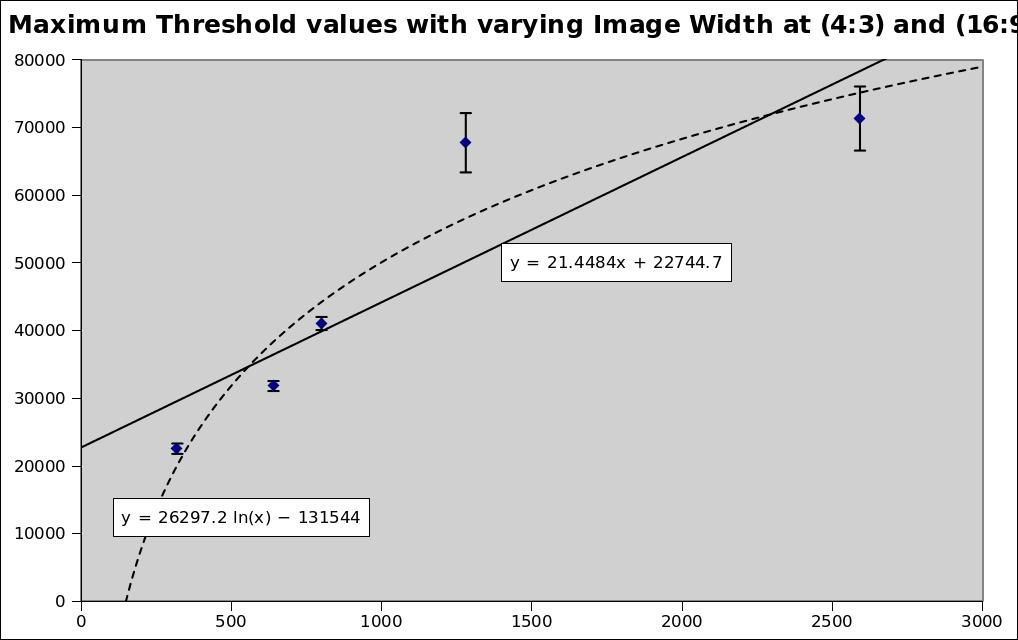
\includegraphics[width=0.7\textwidth]{../images/chart-threshold-with-varying-image}
	\end{center}
	\vspace{-15pt}
	\caption{}
	\label{chart:thresholds}
	\vspace{-10pt}
\end{wrapfigure}

As can be seen in Chart~\cref{chart:thresholds}, two trendlines have been plotted - a linear one, as well as a more relevant logarithmic trendline because the threshold for 0x0 image sizes should tend towards 0, and not have a y coefficient.\\
It should be noted that the standard deviation in the average threshold grew as the image size grew, meaning that this was not the most accurate scale for determining a threshold. I did try setting a threshold with image size using the formula of:\\
 Thresh = 26297*ln(image\_width) - 131544(+10000 as a max limiter),  giving appropriate theshold sizes of:\\
30145 (320), 48373(640), 54241 (800), 66600 (1280), 85155 (2592).\\
This method did work, but there were a fair few amount of false positives being flagged.
%DISPLAY FALSE POSITIVE IMAGES WITH LOTS OF SCATTE\\
\\The random scatter of pixels between static frames is caused by Noise, and I needed to find a way to get rid of it.

\subsection{Noise}
\subsubsection{Thermal Noise, CCD clocking up/down}
\paragraph{Oversaturation, filtering, compression}

\subsection {Noise Removal}
\subsubsection{Running Average}
In this method, a reference frame is created by capturing a quick succesion of frames. The pixel values from these frames are added to an accumulator and then divided by the number of frames  
\footnote{CImg facilities this very easily by using standard operators to perform operations over all pixel values.
\\ E.g.  CImg\(\langle\)T2\(\rangle\) average =  (CImg\(\langle\)T1\(\rangle\)one + CImg\(\langle\)T1\(\rangle\) two + CImg\(\langle\)T1\(\rangle\) three) / 3; \\
Where: sizeof(T2)\(\rangle\)sizeof(T1).
\\The size of the image types is significant. It should be noted once again that greyscale image sizes are 8-bit unsigned chars with a maximum and minimum values from 0 to 255, so appending a series of pixel values will result in in values that overflow this range. For this reason, the accumulator needs to have pixel sizes that can contain accumulated pixel sum amounts. In this project the accumulator had long (64-bit) pixel values, and were then normalised in [0,1] colorspace when being assigned to the reference frame.}
 
This 'average frame' now becomes the reference image which all incoming frames are now checked against it, as shown the pesudo code below

\begin{frame}[fragile]
	\vspace{-20pt}
	\lstinputlisting[title=\textbf{Source Code: UpdateReference.pseudo}]{../Code/pseudo/updatereference1.pseudo}
\end{frame}

The reason a method like this is used to reduce noise is because the noise over several frames is 'blurred' out and only the significant motion stands out. This blurring effect reduces the amplitude of the random noise, since it is unlikely that a noisy pixel will occur at the same position across all frames , thus for 100 frames: \\\t if a noisy pixel occurs at position [10,5] with a value of 255 (white), then this will be reduced to a pixel value of 3 after the running average method is applied, since due to the arbitrary nature of noise, the noisy pixel is unlikely to occupy the same pixel position in successive frames. Pixels which retain their values over more than a few frames can then be said to be significant, since it is unlikely for random noise to strike the same pixel twice (unless the scene is generally very noisy)\\
It should be noted that this blurring effect occurs for all pixels and not just noisy ones, and so there is a slight - but generally acceptable - reduction in sharpness of the image.\\
The amount of noise reduction is proportional to the square-root of the number of frames being averaged, so in the 100 frame example the reduction of noise would be a factor of 10.

\paragraph{
In the pseudocode below, the current frame is subtracted from the reference frame, and if the non-zero pixel count from the subtracted frame is over the (new) threshold amount, then the movement is flagged and the reference frame is updated by another quick burst of frames.
}
\begin{frame}[fragile]
	\lstinputlisting[title=\textbf{Source Code: accumulator.pseudo}]{../Code/pseudo/accumulator1.pseudo}
\end{frame}
\paragraph{Note that the updateReference function has changed so that the reference frame is the accumulated normalisation over any number of frames. \\
All frames are normalised to [0,1]  binary colorspace, as this flattens the image and produces less diference between one frame and the next, which helps distinguish where movement has occured.
}
\paragraph{As shown in ~\cref{accumst} a static scene shows very little difference from one scene to the next so that the image is coherent. For a dynamic scene, \cref{accumdy} shows a wildly different image with traces of many different scenes superimposed.
\\This approach introduces the concept of having a background or reference, since by the subtraction method of motion detection we would have no knowledge of the background since we would only be comparing two temporally adjacent frames.
}
\begin{wrapfigure}{R}{0.45\textwidth}
	\vspace{-30pt}
	\begin{center}
		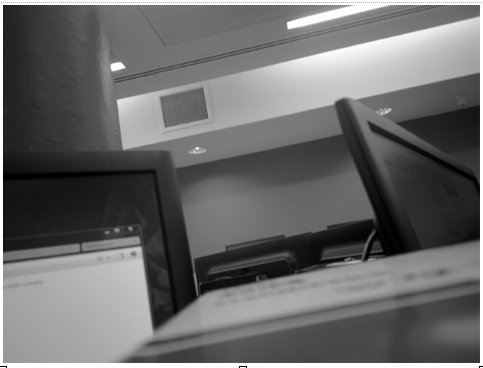
\includegraphics[width=0.45\textwidth]{../images/accumstatic}
	\end{center}
	\vspace{-20pt}
	\caption{10 frame accumulation for static scene}
	\label{accumst}
	\vspace{10pt}
	\begin{center}
		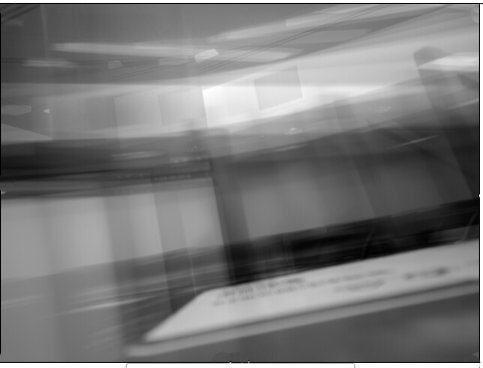
\includegraphics[width=0.45\textwidth]{../images/accumdynamic}
	\end{center}
	\vspace{-20pt}
	\caption{10 frame accumulation for dynamic scene}
	\label{accumdy}
	\vspace{30pt}
\end{wrapfigure}
Running repeated tests under this model confirms that the threshold value is much lower than it used to be due to the reduction in the noise, but there is still large growth of standard deviation as the image size increases. This is due to the scatter of noise that still persists 
\begin{wrapfigure}{R}{0.35\textwidth}
	\vspace{-40pt}
	\begin{center}
		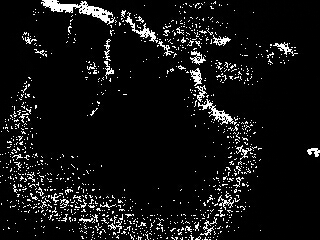
\includegraphics[width=0.35\textwidth]{../images/scatter1}
	\end{center}
	\vspace{-30pt}
	\caption{Scatter of noise for a 1-frame running average}\label{img:scatter1}
	\vspace{10pt}
	\begin{center}
		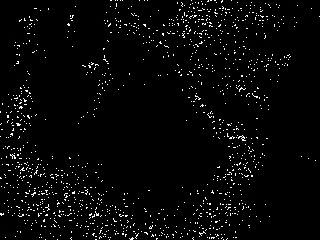
\includegraphics[width=0.35\textwidth]{../images/scatter2}
	\end{center}
	\vspace{-20pt}
	\caption{Scatter of noise for a 10-frame running average}\label{img:scatter2}
	\vspace{-20pt}
\end{wrapfigure}

the images, even averaging over 30 frames or more \footnote{Averaging over higher even using the fastest frame times causes a significant delay in the application and can also cause segmentation faults.}
leaves noise behind which are counted as non-zero white pixels in a normalised image.

The images above show how the running average method reduces the localised noise within certain regions, but increases the overall scatter of the noise as it accumulates around certain individual pixels as it is 'flattened' over several frames.\\\linebreak
\pagebreak In \cref{img:scatter1} the noise is clustered together and makes up a significant part of the static image. But in \cref{img:scatter2} the noise is much more sparsely spread and most of the noisy white-pixels are surrounded by empty neighbours.\\

Clearly another technique is needed to smooth the images so that sparse pixels surrounded by emptiness can be ignored and not contribute to the threshold count. Such techniques are called {\bf morphological operations}

\subsubsection{Image Morphology}
Another way to reduce noise in an image is to 'smooth out' random white pixels, so that an image dotted sparsely with noise is converted into an image that contains only the most concentrated of clusters.  To do this one needs to smooth the pixels.
In binary colorspace, smoothing a pixel requires considering the values of the neighbouring pixels. If pixel A has 8 neighbours (adjacent/diagonal), then the 0 or 1 value of pixel A is determined by the value of its neighbours.\\
To {\bf Dilate} a pixel is to set its value to 1 if all (or most) of it's neighbouts are also 1.\\
To {\bf Erode} a pixel is to set its value to 0 if all (or most) of it's neighbours are also 0.\\
A simple example is shown below:
\begin{center}
\begin{frame}
.\\
Original\tab	Dilate\tab	Erode\tab\\
\tiny{
0000000\tab	0000000\tab	0000000\\
0000000\tab	0011100\tab	0000000\\
0011100\tab	0111110\tab	0011100\\
0010100\tab	0111110\tab	0011100\\
0011100\tab	0111110\tab	0011100\\
0000000\tab	0011100\tab	0000000\\
0000000\tab	0000000\tab	0000000\\
}
\end{frame}
\end{center}

To specify the level of smoothing, one needs to consider a {\bf kernel}
\paragraph{In algebra a kernel is a linear operator which performs an operation upon a set of data. In imaging, the data is a matrix of pixels, and the operator is a much smaller matrix of predefined size that acts as a structuring element and performs basic matrix superimposition upon the pixels and it's neighbours. \\
A kernel is therefore the size of the neighbourhood being considered when performing Erosion or Dilation operations. Generally a kernel is an nxn square matrix applied as a mask over each pixel, but it is not bound to this shape and can take any nxm best suited.
A 2x2 kernel will consider the three surrounding neighbours of a pixel, a 3x3 kernel will consider 8 surrounding neigbours of a pixel, a 4x4 kernel will consider 15 surrounding neighbours and so on.
}
\paragraph{For  image processing, a kernel normally comes in two shapes: A Diamond structure or a Square structure. A diamond structure kernel is the least discriminating as it considers only the genreally adjacent neighbours of a pixel and not the corners. A square structure  is the most discriminating as it considers all the neighbours and will only affect the centre pixel if all the neighbours confirm to the rule of the operation.
\\
Diamond kernels produce softer edges on images, and Square kernels produce blocky edges. Generally a square kernel is likely to remove more pixels than a diamond will, though a diamond is more likely to preserve the overall shape of the image.
}
\paragraph{A common technique in image smoothing is to perform 'opening/closing', which is simply an dilation followed by an erosion. This accentuates the important parts of the image and also filters out any sparse pixels.}

\subsubsection{Experiments}
\paragraph{As of version 1.1.2, CImg comes with its own dilate and erode functions, and the kernel can be specified by a simple array. A series of tests were performed:
}
Starting image \cref{img:uneditsub1} shows the difference between two  completely different frames:
\begin{figure}[H]
	\hspace{0.24\textwidth}
	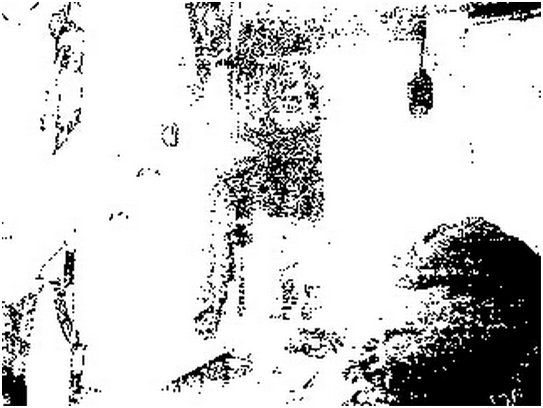
\includegraphics[width=0.5\textwidth]{../images/ImageOps/uneditedsub}
	\caption{White pixel count of 87516.}
	\label{img:uneditsub1}
\end{figure}

\pagebreak
{\hspace{-20pt} \bf Test 1:}{\underline{White pixel count variation with repeated Erosion/Dilation using a 2x2 mask}}\\
(See the appendix for the code used.)
\begin{figure}[H]
	\vspace{-10pt}
	\begin{center}
		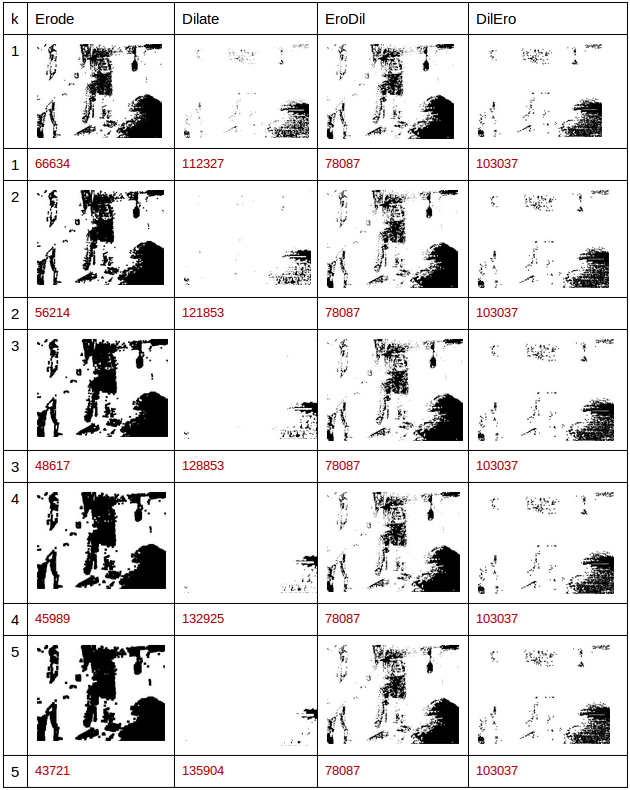
\includegraphics[width=0.8\textwidth]{../images/ImageOps/test1}
	\end{center}
	\vspace{-20pt}
	\caption{\small Erosion, Dilation, Erosion followed by Dilation, and Dilation followed by Erosion all repeated k times}
	\label{img:erode1}
	\vspace{-10pt}
\end{figure}

As we can see from \cref{img:erode1} -- repeated uses of Erosion/Dilation (or vice versa) does not affect the white pixel count for repeated usage as they do independently.
\\It is interesting to note that EroDil produces a more solid image (i.e. black parts dont have white spots within) than DilEro. This is most likely because the sparse pixels have been filtered out first, and then accentuated. If it were the other way then the sparse pixels would have been accentuated first by the dilation, and then persisted under the erosion.
One thing to note is that not much has been clustered. It seemed like the 2x2 mask was too small and so I repeated the experiment with increasing mask sizes\\

{\hspace{-20pt} \bf Test 2:}{\underline{White pixel count variation with repeated Erosion/Dilation using an increasing mask}}\\
The same starting image is used, as loaded in from a previous save.
\begin{figure}[H]
	\vspace{-10pt}
	\begin{center}
		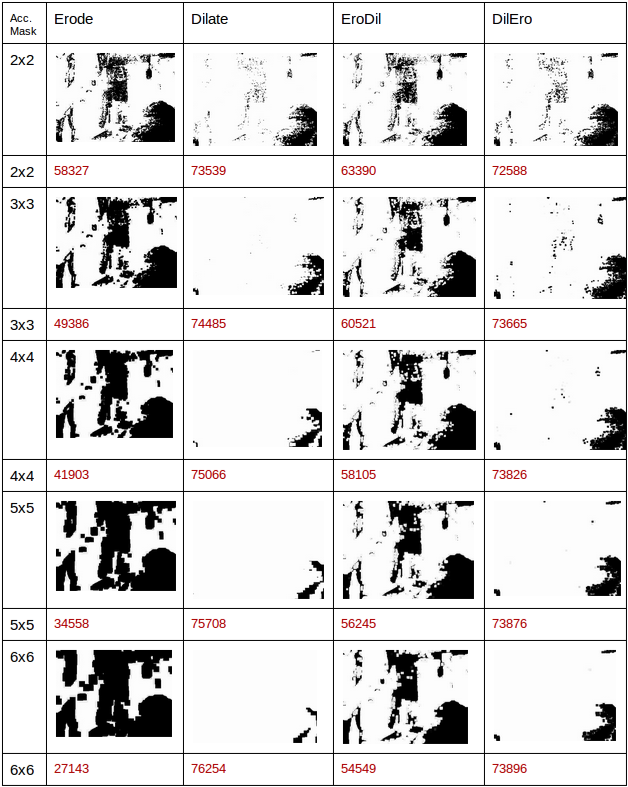
\includegraphics[width=0.8\textwidth]{../images/ImageOps/test2}
		\label{img:erode2}
	\end{center}
	\vspace{-20pt}
	\caption{Erosion, Dilation, Erosion followed by Dilation, and Dilation followed by Erosion using kxk mask size}
\end{figure}
As expected the white pixel count increased in the EroDil and DilEro techniques with increasing square masks, however EroDil seemed to give the best quality bunching out of all the technique. Dilate by itself seemed pretty effective too, but this alone would not remove noise effectively. Dilero had to be dropped as useful image processing method since it seemed to be removing significant parts of the image and not retaining the overall blobby structure.

{\hspace{-20pt} \bf Test 3:}{\underline {Seeing how white pixel count varies with repeated seperate calls to Erosion and Dilation}}
\begin{figure}[H]
	\vspace{-10pt}
	\begin{center}
		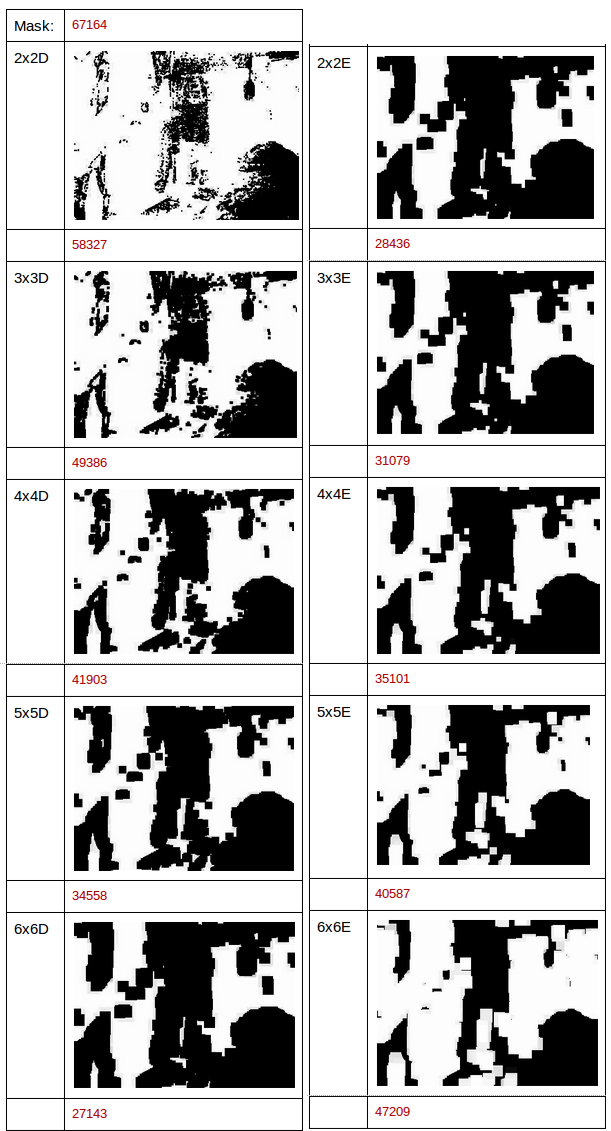
\includegraphics[width=0.6\textwidth]{../images/ImageOps/test2A}
		\label{img:erode3}
	\end{center}
	\vspace{-20pt}
	\caption{Dilation and Erosion varying with a kxk mask}
\end{figure}

As expected, the white pixel count diminishes under the repeated Erosion calls, then grows under the repeated Dilation calls. Clearly using these techniques seperately serves no purpose other than accentuating white and black respectively. However combined together into an EroDil method, the structure of the image itself is accentuated and not just one specific color as shown in \cref{img:erode4}
\begin{figure}[H]
	\vspace{-40pt}
	\begin{center}
		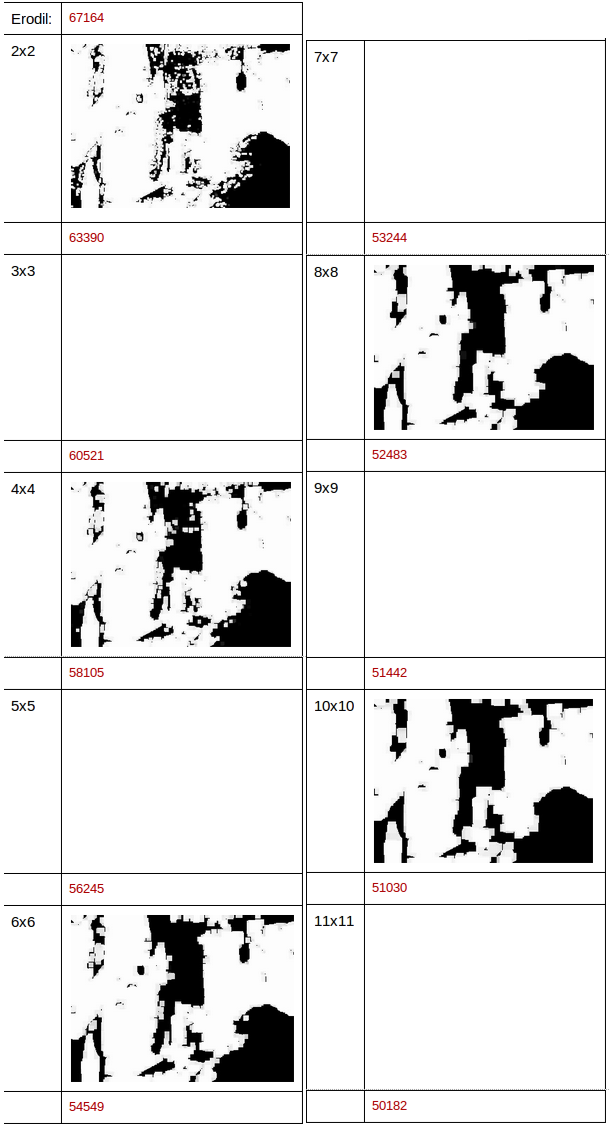
\includegraphics[width=0.6\textwidth]{../images/ImageOps/test2B}
	\end{center}
	\vspace{-20pt}
	\caption{Dilation and Erosion varying with a kxk mask}
		\label{img:erode4}
\end{figure}

The erodil images were taken at bi-intervals, but the intermediate mask sizes were performed.  EroDil increases the white pixel count, but gradually -- and this makes sense since the image is mostly white, so the increasing white pixel count is representative of this. In terms of tidiness, EroDil seems to produce a smoother image, and gives a white pixel count that is closer to the true white pixel count of 67164, than anything that Eroding or Dilating could do by themselves.

\pagebreak
{\hspace{-20pt} \bf Test 4:}{\underline {Seeing how White-Pixel count varies with increasing Mask Size using EroDil method:}}
\begin{figure}[H]
	\vspace{0pt}
	\begin{center}
		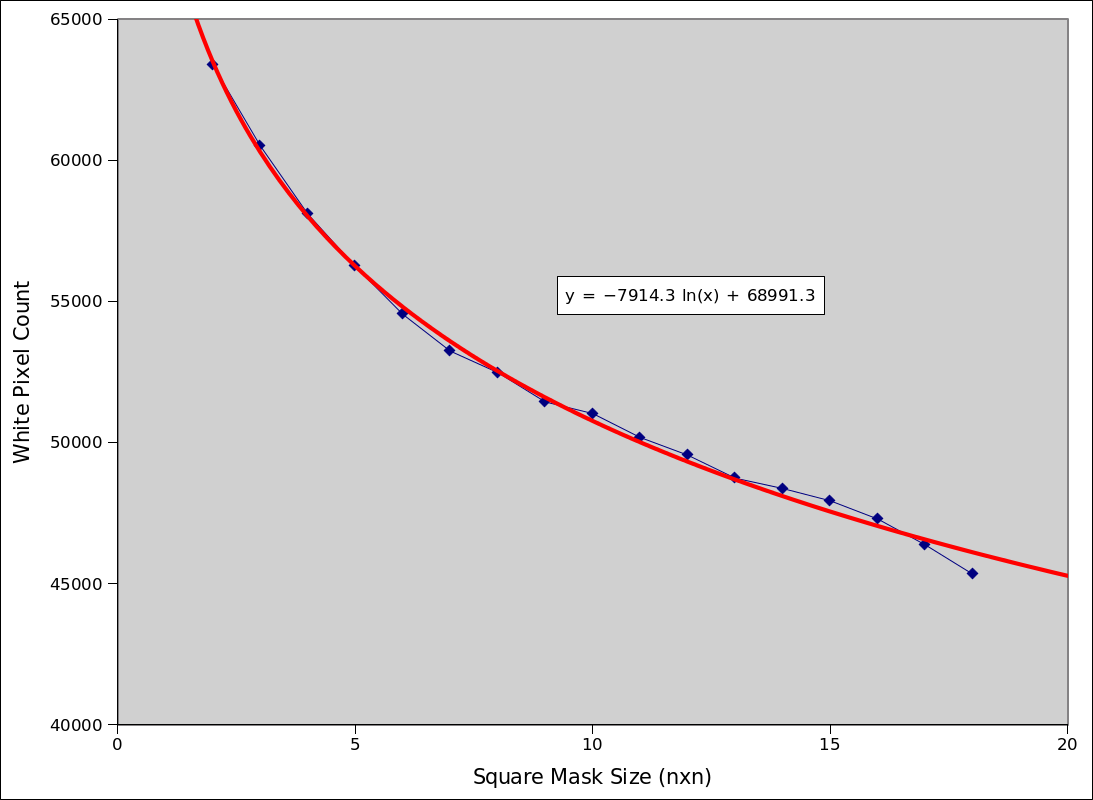
\includegraphics[width=0.8\textwidth]{../images/ImageOps/chartMask}
		\caption{}
		\label{img:maskChart}
	\end{center}
\end{figure}
As seen in \cref{img:maskChart} the white-pixel count follows a downward logarithmic trend that is very well approximated by the equation:\\
WhitePixelCount = 68991.3 - 7914.3 ln(MaskSize)

It should be well noted that applying a larger mask filter to an image that has been affected by a smaller mask filter, is {\bf exactly the same} as simply just applying the larger filter.  In my code in the appendix what I tended to do was repeatly loop over and update the existing image with each increasing mask, such that the input for mask B would be the output for mask A, where BxB \(\rangle\) AxA.  The reason why I did this was to prevent the application from constantly replacing the current image in the memory, rather than having to duplicate from the original for each mask.

Various other tests were performed: See Testing section in the appendix, but these core 4 tests demonstrated all I really needed to know about opening/closing an image - i.e. As the mask size increases the white-pixel count converges downwards at an ever decreasing rate. Using this knowledge I then set on detecting different kinds of movement.

\subsection{Movement Types}
I broke movement down into 5 different types:  Scene change (80\% of the image), Medium movement (40\%), Small movement (10\%), and Tiny movement ( less than 3\%).

For scene changes, I moved the camera from one position to another between frames. As implied in Mask sizes have to get very large (to the same order as the image dimensions!) before a subtracted image for differing scenes can  fully converge to a single colour:

%LARGE
\begin{figure}[H]
        \vspace{-20pt}
        \begin{center}
                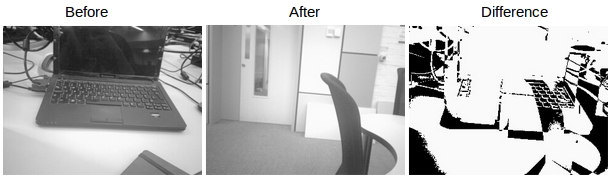
\includegraphics[width=0.7\textwidth]{../images/ImageOps/Diff1}
                \label{img:diff1}
        \end{center}
        \vspace{-20pt}
        \begin{center}
                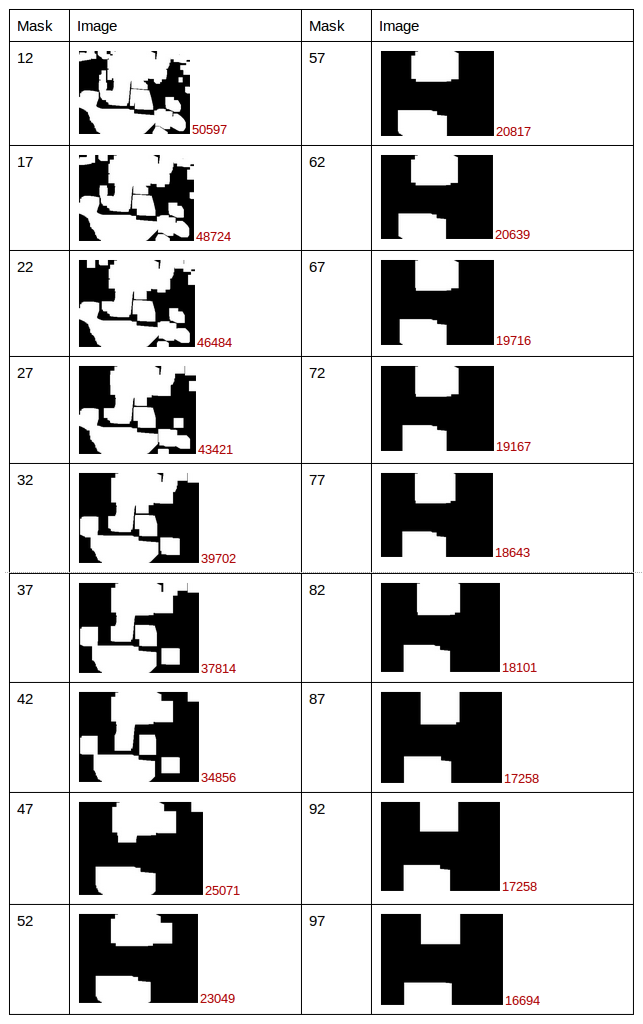
\includegraphics[width=0.7\textwidth]{../images/ImageOps/Diff2}
                \label{img:diff2}
        \end{center}
        \vspace{-20pt}
        \caption{Base image undergoing EroDil to large mask sizes. Even a 97x97 mask couldn’t fully vanish the scene}
	\vspace{-40pt}
\end{figure}

Since the mask size required to completely ignore a scene change is probably on the same order of the dimensions of the image.  To ignore a scene change, it seemed apt to simply set a lower limit on the White Pixel count (e.g \(\langle\)25000 is good enough).
\\To detect medium movement I placed the camera to face the screen of a computer and dragged a window across the screen. \cref{img:medium} shows the drop in white pixel count as the Mask size increased until vanished completely for a 16x16 mask size
%MEDIUM
\begin{figure}[H]
	\vspace{-12pt}
	\begin{center}
		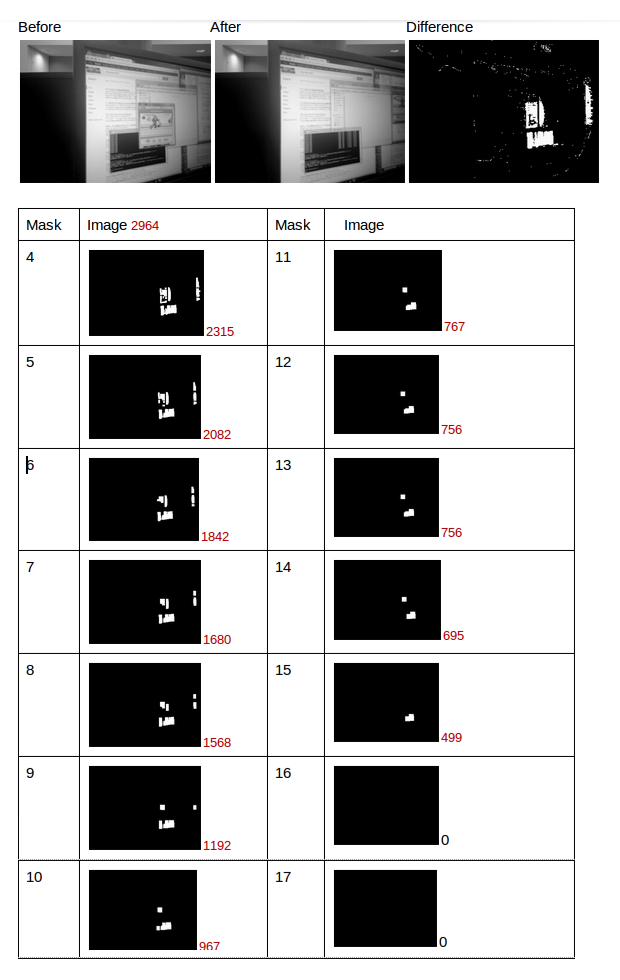
\includegraphics[width=0.8\textwidth]{../images/ImageOps/LARGE}
	\end{center}
	\vspace{-30pt}
	\caption{Medium movement, ignored at 16x16 mask}
	\label{img:medium}
	\vspace{-40pt}
\end{figure}

To detect small movement I repeated the same experiment, but this time made the contents within the window change (i.e. a movie) without moving the window itself.  A small window in the computer screen will change between the images, but the overall scene wont change. This test will determine for which mask sizes movement is no longer detected.
For filename reasons, the masks increase in multiples of (4*i)+2  (e.g 2,6,10,14,18,etc). \Cref{img:small} shows that movement is ignored up to a mask size of 5x5:
%SMALL
\begin{figure}[H]
	\vspace{30pt}
	\begin{center}
		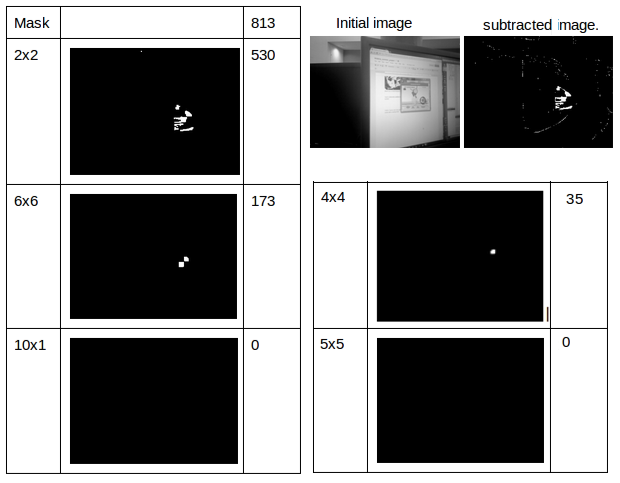
\includegraphics[width=0.9\textwidth]{../images/ImageOps/SMALL}
	\end{center}
	\vspace{10pt}
	\caption{Small  movement, ignored at 5x5 mask}	
	\label{img:small}
	\vspace{20pt}
\end{figure}
\pagebreak
To  detect tiny movement I placed a single blinking cursor on the screen. The experiment was repeated twice.
\begin{figure}[H]
	\vspace{-10pt}
	\begin{center}
		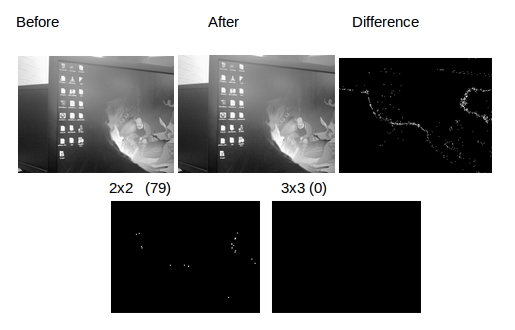
\includegraphics[width=0.8\textwidth]{../images/ImageOps/CURSOR1}
	\end{center}
	\vspace{-20pt}
	\caption{Blinking Cursor}
	\label{img:curse1}
\end{figure}
\begin{figure}[H]
	\begin{center}
		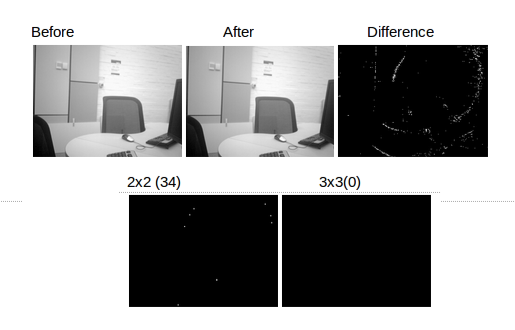
\includegraphics[width=0.8\textwidth]{../images/ImageOps/CURSOR2}
	\end{center}
	\vspace{-20pt}
	\caption{Static scene - Noise}
	\label{fig:curse2}
\end{figure}

As shown in \cref{img:curse1} and \cref{fig:curse2}, something appears to be picked up for a 2x2 mask, but both are ignored for a 3x3 mask. This means that tiny movement is of the same order as noise, and so a 3\% difference between images cannot be accurately flagged as movement.



\section{Threads}
Threads are processes that appear to run at the same time to other processes. On multi-core devices, the illusion is true: two processes genuinely can run in different cores at the same time. On a single-core device such as this, the illusion is false: the OS scheduler switches between different processes to allocate time-slices to each process at regular intervals.\\
\\In mobile applications, threading is necessary as often a background task needs to be run which will halt the user interface until the task is complete. In the first draft of my application, this was the case - the buttons and widgets that controlled the camera execution would become unresponsive until the camera had finished its process, where control would then flow back to the user-interface.
\\This is fine in the situation that the user presses a button and walks away from the phone, but if more control is desired (i.e. the ability to terminate the application while it is running) then threading is necessary.

\subsection{Camera Thread}
Originally my Camera Class was simply an object class. I would create a Camera object, and tell it to perform functions, and then delete it when it was no longer needed. To place it into a thread, I had to change it from an QObject class to a QThread class. In Java this would be a problem, since only single-parent inheritance heirarchies are permitted, and so the class would lose it's object methods (clone(), ~delete()), but in C++ a class can have many parents, and so I was able to inherit both QObject and QThread classes.
However, this caused many conflicts as errors sprung up detailing multipled definitions of the same function. By going through the Qt API I discovered that QThread actually already inherits QObject (as do all Q Classes) and so the Object methods that my Camera class originally had would not be lost if I simply inherited from QThread.

QThread has a protected method called start() which is the same as Java Thread's run(), which is a method that must be called to run the thread after the thread object is created. Originally this just performed the standard functions from before:  initialise camera, check for movement, and terminate. But I wanted to be able to stop the thread safely at any point from the UI without crashing the application. In order to do this I had to use Qt's Signals/Slot's framework.

\subsubsection{Signal/Slots}
Signals and slots are a core mechanism in Qt that sets itself apart from all the others. It is essentially a notification framework, so that when Object A performs something then Object B can know about it.  Traditionally, these are enabled through the use of callbacks, where a global pointer to a function is passed between objects to enable communication. However callback's are not very type-safe since the pointer can reference anything and there is no gauruntee that the callback will be called with the correct parameters.

Signal and slots provide an alternative to this. When a particular event occurs in Object A, then A emits a signal for that event. A slot  is then called to handle the signal, where a slot is simply a function which has the extended ability to listen for signals. If Object B has a slot that is paired with a signal from Object A, then  B will run it's slot when A emits its signal.

Pairing signals to slots is a relatively simple process: One simply calls:   connect(ObjectA, SIGNAL(mySignal), ObjectB, SLOT(mySlot)).
It should be noted that this is type-safe, such that the argument of mySignal must be of the same type as the argument of mySlot. Both are void functions.
connect is a function of QObject, and so to enable signals/slots, one must inherit a QObject (or any one of it's subclasses). A Q\_OBJECT macro will then have to be declared in the header file of that class to enable signal/slot functionality. 

Pairing usually occurs automatically: When a button is clicked, Qt creates a slot for it in the source file and the user can then edit the slot to perform some task. The connect:: script is never seen in the source file, but is included in the autogenerated MOC files and so the implementation is seamless.

Custom slots are another story. Though this mechanism is completely native to Qt, it can very temperamental trying to create custom slots. Often you will need to clean, rebuild, make, clean, rebuild, make, and so forth until the custom signal or slot is accepted. This is undoubdetly a bug of Qt and has been reported by previous users: https://bugreports.qt-project.org/browse/QTBUG-17072.

For the Camera thread, I paired a stop button signal from the UI thread with a stop() slot in the camera thread. The stop() slot in the camera thread simply changed a class boolean variable called 'stopNow' to True.  In every function within the camera thread, whenever a loop occurred  stopNow!=True would be a condition that would terminate the loop. This would exit the function early and cause the Camera Thread to perform its Deletion function and stop the camera thread safely without crashing the application.

As I got more used to the mechanism, I started to harness it more effectively to the point where I began passing whole images from the camera thread back to the UI. A useful feature of signals and slots is that it's not just a flagging system, but can also transport data between threads.  To pass a whole image, one simply defines the argument of the Signal in the camera thread as having an argument of type FCam::Image, then when one wants to emit the signal, one simply calls' emit mySignal(image\_arg)'. In order for Qt to recognize the type of object being passed between threads, the argument type needs to be registered via 'qRegisterMetaType\(\langle\)FCam::Image\(\rangle\)("FCam::Image")'.

Passing whole images can be wasteful however, since it requires cloning the current image to memory and passing it to the UI. For small images this is not much of a problem, but for large image sizes this can cause significant overhead since cloning will take a long time and two copies of the same image will take up a significant amount of memory. Instead I passed a reference to the image '\&image'. This is risky because that reference may refer to an address where the image used is to be hed until another thread changes it. Technically a mutex variable would prevent the camerathread from changing the address of the image while the Ui thread is still reading it, and Qt comes with it’s own QMutex object which can lock and unlock critical sections of code so that only one thread can be performing something critical to the same object at any one time.

I dedided against using this since I managed to get a stable application by specifying that the new frame was to be at a constant address and that the newImage signal was also constant ‘const FCam::Image’. This made sure that I no longer needed to delete frames after I had processed them, since any new frames would simply be loaded into the same address overwriting the old frame. The only time I needed to delete an image was on thread exit and in the long intervals between frames. This greatly saved on system resources and reduced the size of the signal.

The newImage signal was only ever emitted when movement occurred, otherwise it lay dormant between regular unmoving frames.
To save further overhead, Qt allows for signal/slot pairing to be unpaired with ‘unconnect’, so I created a tickbox in the Ui thread which when unticked would unpair the newImage signal with the slot, and when ticked would pair the two.

\subsubsection{QImage, QPixMap, and CImg}
Once I was sure that the image was being recieved in the UI, I needed to display it in my main window. This proved harded than originally anticipated. To display an image in Qt, one needs to create a QLabel widget and apply a pixmap to it. A pixmap (or QPixmap) can be created from a resource file specified at build time, or can be specifed from a QImage. Since a QImage is merely a container and does not need to be an absolute resource, I decided to convert CImg to QImage. 

My initial attempts brought about images that were misaligned, badly coloured, and often times blank. To get the root of the problem I attempted many different size configurations:
\begin{frame}[fragile]
	\vspace{-20pt}
	\lstinputlisting[title=\textbf{Source Code: shell1.cpp}]{../Code/qpix/shell1.cpp}
	\label{code:shell1}
\end{frame}
This attempted to make a thumbnail out of the image recieved from the signal and convert it into the appropriate format in a QImage. This would then be converted into a pixmap and assigned to Label for dispaying.

Arguments from commandline were passed in generated from a shell script to vary the image size slightly so that both the width and height of the original image were divided a ‘mod’ factor and ‘offset’ by a certain amount, as well as being offset from the top left of the image by pixel amounts of ‘top’ and ‘left’, varying from 0 to 50 in increments of 1. ‘offset’ was varied from 0 to 100 in steps of 10, and ‘mod’ was varied from 1 to 3 in increments of 0.3.

Needless to say the script took a long while to finish executing, but I wanted to be as thorough as possible in finding a suitable image size and alignment that displayed a usable image. Most of the images came out horribly deformed and squished, except those that had a mod value of 2 and offset 0. As shown in \cref{fig:shell1} I also quickly learned that the top and left arguments simply state where the starting pixel to start drawing the image should start.
\begin{figure}
	\begin{center}
		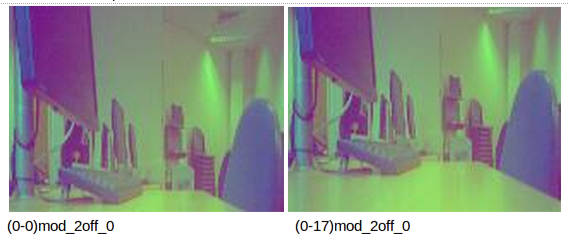
\includegraphics[width=0.8\textwidth]{../images/qpix/shell1}
	\end{center}
	\vspace{-20pt}
	\caption{Two usable images with width and height divided by 2. The left has no offsets, but the right has a vertical offset of 17 pixels. }
	\label{fig:shell1}
\end{figure}

It seemed strange that the QPicture needs image boundaries at half the actual image size it is containing, but despite scouring through the QPicture API I could find no reasoning for it. Nonetheless, a usable image was found, I just needed to adjust the color channels for it.
To do this I adjusted the shell script from \cref{code:shell1} to adjust just the Image format and size, just in case size was somehow dependent on the format (it shouldn’t be since they are two completely different entities, but I wanted to cover all bases).
\pagebreak
\begin{frame}[fragile]
	\lstinputlisting[title=\textbf{Source Code: shell2.cpp}\label{code:shell2}]{../Code/qpix/shell2.cpp}
\end{frame}
This resulted in yet another flurry of badly aligned images as shown in \cref{fig:shell2}
\begin{figure}
	\begin{center}
		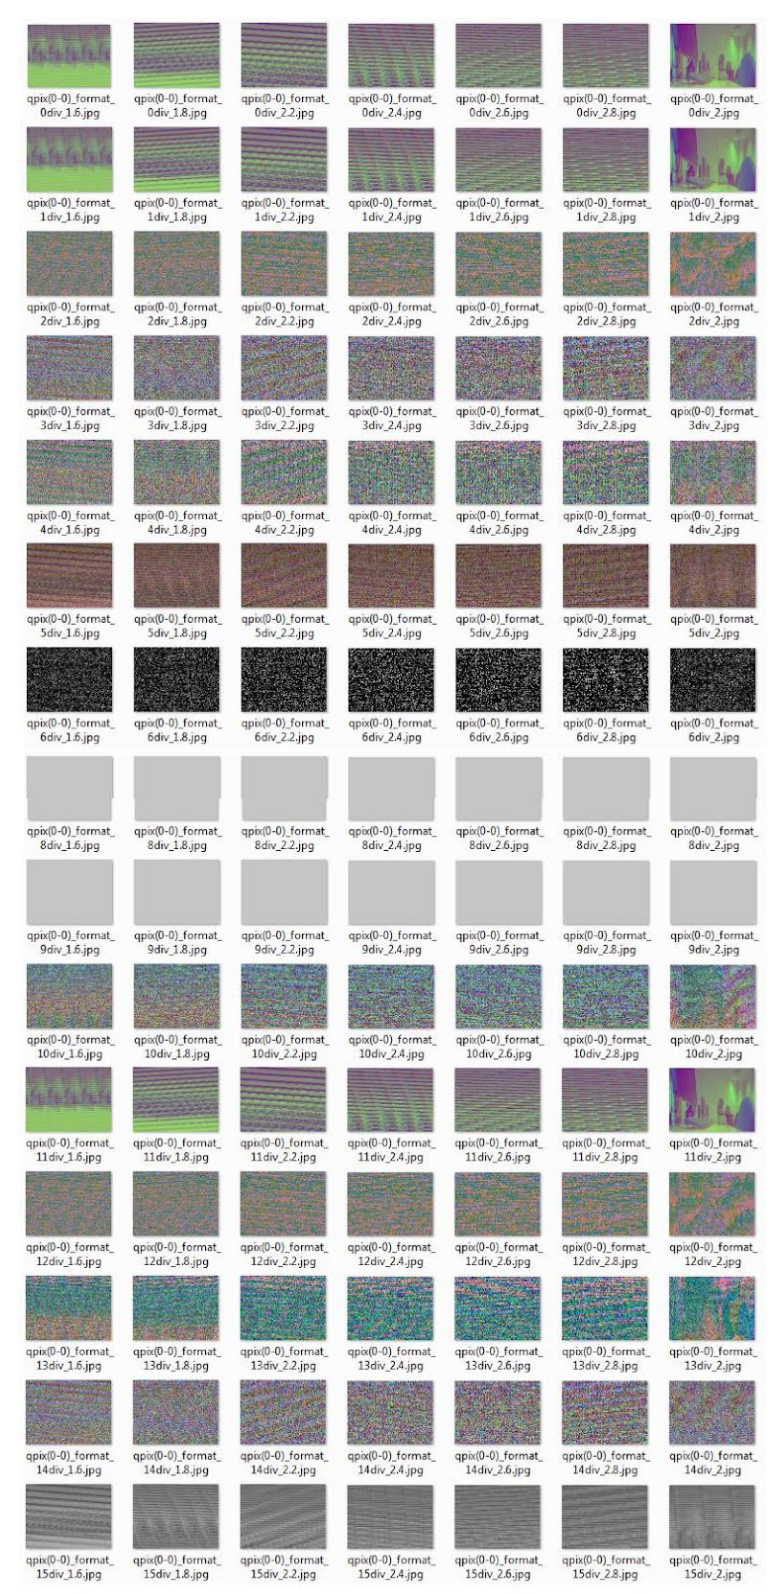
\includegraphics[width=0.8\textwidth]{../images/qpix/shell2}
	\end{center}
	\vspace{-20pt}
	\caption{Usable images are where ‘div’ amount equals 2 and format is 0, 1, or 11}
	\label{fig:shell2}
\end{figure}
Out of all the images in \cref{fig:shell2} , only three were actually usable - all ocurring where the image dimensions were halved. This put to rest my earlier unfounded suspicions that image size was affect by the image color format. The usable image formats were QImage::Format\_ARGB32, QImage::Format\_ARGB32\_Premultiplied, and QImage::Format\_RGB32.  Once again, the color was slightly off again, appearing more magenta than it actually was.

Wondering if the problem was to do with RGB channels being in different order for QImage’s (the idea came to me after remembering that OpenCV’s IPLImage format was by default BGR), I swapped the blue and red channels using QImage’s swapRGB() function. To my surprise this produced very little difference in the outputted images as shown in \cref{fig:swaprgb}
\begin{figure}
	\begin{center}
		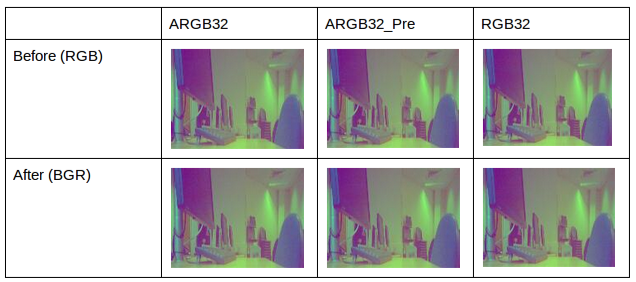
\includegraphics[width=0.7\textwidth]{../images/qpix/swaprgb}
	\end{center}
	\vspace{-20pt}
	\caption{}
	\label{fig:swaprgb}
\end{figure}

 The difference between RGB32 and ARGB32 is that the latter has an Alpha channel which is used for image types that support transparancy such as PNG. The Alpha channel itself holds the pixel value of the pixel behind the current image itself, enabling it to seem as though it is transparent.  The premultiplied version is almost identical to the standard ARGB32 format, but the red green and blue channels are ‘premultiplied’ by the alpha channel so that the image can softly fade into transparency instead of the transparency suddenly cutting into the image. It produces very gradual and precise images, but with lots of processing overhead.

Considering how my application has no need for transparency I dropped these two formats to save image storage overhead, leaving me with RGB32. 

This in itself was wasteful, since in CImg the format I was using was an 8-bit unsigned format, and so the image I should be passing should be the 8-bit CImg. Unfortunately Qt did not agree with me on this point since in order to pass it as a valid signal I would have to include the CImg header file in the header file of my camera class. Qt did not like this and only let me place the CImg header in the source file, and so I was not able to pass the CImg has the signal.

This meant I had to use FCam, and since I was only passing a reference to the FCam::Image, it made no difference how big the actual image was or what format it was. In fact it would have wasted more processing time, converting the FCam::Image into an 8-bit format to then be signalled. So instead I used the RGB32 format, a format that was 4 sizes larger than the 8-bit unsigned format I was using with CImg. 

As of yet I have not found a way to display a movement image without the color problem, but this is not something that is essential to the backend functionality of the app, and so it is something that will be rectified as a hotfix in future releases.

\subsection{Email Thread}
A major selling point of the application is the feature to email the user in real time upon movement detection. This ensures that the user does not have to be within the same vicinity as the phone to be notified that movement has occured, and is therefore a useful tool in security and privacy concerns.

Before starting the camera the user can choose to set an email address, message, subject, and can also choose to attach an image to the email, so that they can catch the latest image with the movement occuring within it. As a burglar alarm, this would be the method of catching the culprit red-handed so to speak.

In order to do this a framework needed to be used to send the email.
Qt provided an example in version 3.x of a class that could send emails to a specified SMTP server using QTCPSocket objects http://lists.trolltech.com/qt-interest/2006-10/thread01158-0.html, but this was dropped in recent versions of Qt and despite trawlng the forums very few users had managed to use this class file effectively in Qt4.7. So I was unable to use this framework to send an email. This was not neccesarily a bad thing, since the SMTP server would have to be defined by me and I would have had to have some kind of address book of every SMTP address in order to send an email to gmail or hotmail or whatnot.

Instead I looked at the phone itself for a framework.  QtMobility looked promising, but several problems were reported for Maemo http://www.developer.nokia.com/Community/Discussion/showthread.php?201846-Sending-Email-Using-Qt-Mobility which was confirmed by several users, and so I had to look at another alternative.

A veteran user on the Maemo community site had written an app called ‘mailcmd’ http://talk.maemo.org/showthread.php?t=82918 that was a simple commandline utility that sent emails using the default email account setup on the phone. It even allowed for attaching images and the sheer simplicity of its usage was exactly what I needed.

This added the ‘mailcmd’ dependency to my project, but it is a small package and I don’t think users would mind too much. I created a class file that inherited a QThread which ran a QProcess to execute the mailcmd command in a new thread.

This means that any time during the application, there will be at maximum three threads running: UI, Camera, and Email. Email needed to be run on it’s own thread, otherwise the camera thread would hang between frames as it waits for confirmation of the email to be sent. I wanted the application to be as responsive as possible and so I created a seperate thread for Email to avoid this problem.

\subsection{Optimisations/Error Proofing}
Autoexpose on updateReference (drastic changes in brightness levels), interval scaling, lens open check.
\subsubsection{Kernel Compatibility}
Early on in the development of the app, I came across problems where the FCam driver would not initialize properly, and no warning messages were given. Upon reboot it sometimes worked, but it would tend to work the most when I used the default phone kernel PR-1.3.

For this reason I enabled a kernel check at the start of the Camera thread which would issue out a warning whenever a kernel different from the PR-1.3 kernel was being used. This was a simple shell call to ‘uname -r’. However the root of the problem turned out to be that I was not initializing the camera properly when I started the thread, and so when I fixed this problem, the kernelCheck function became redundant and I deleted it from the source.

\footbibliographystyle{plain}
\footbibliography{citers}



\end{document}